\lettrine[lines=2,slope=0pt,nindent=4pt]{\textbf{I}}{n} this fifth part of the document,
the flow pattern changes completely compared to the two previous parts since here are considered turbulent flows.
Let us remind that a flow is considered as turbulent when the Reynolds number is greater than 2000.
This critical Reynolds number corresponds to the moment when the viscous forces are no longer strong enough
to absorb the vortices. Fluid motion is characterized by chaotic changes in pressure and flow velocity.
The flow has a whirlpool character at all points: eddies whose size, location and orientation vary constantly.
Turbulent flows are therefore characterized by a very disordered appearance, behavior that is difficult to predict,
and the existence of numerous space and time scales.\newline
In this version of the report, two cases are studied:\vspace*{0.3cm}\newline
\hspace*{0.5cm} $\bullet$ Turbulent flow in a 2D diffuser with the $k-\epsilon$ model\vspace*{0.3cm}\newline
\hspace*{0.5cm} $\bullet$ Mixing length in 2D and 3D VEF-plane channel\vspace*{0.3cm}\newline
This part will be enriched in a following version with, in particular, a case in 3D.\vspace*{2cm}\newline
\begin{center}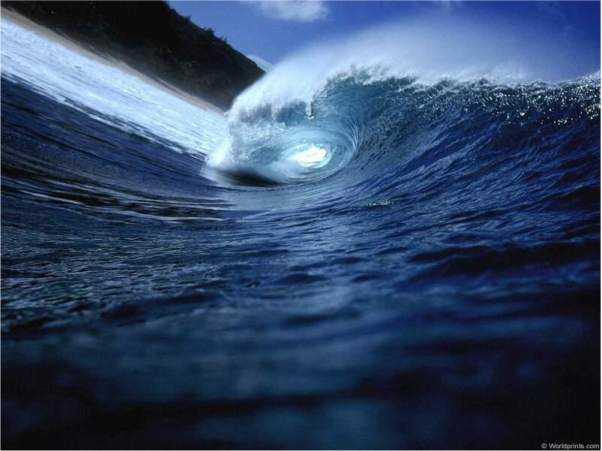
\includegraphics[width=12cm]{tools/mer_turb.png}\end{center}
